In questa sezione sono riportati i risultati del confronto tra le normali climatiche di stazione e quelle ricostruite con approccio \emph{leave one out} e interpolazione LWLR secondo il metodo usato nel lavoro del 2014. L'obiettivo è ottenere una stima preliminare sulla fattibilità della produzione di un dataset grigliato delle normali interpolate e sondare i fattori che influenzano le prestazioni del modello in questa fase iniziale. In quanto segue, con il termine ``BIAS'' si indica la differenza tra le climatologie da modello e da ossevazioni, mentre con ``MAE'' ed ``RMSE'' rispettivamente la media del valore assoluto del BIAS e la radice della media dei BIAS quadrati.

\begin{table}[ht]
  \centering
  \begin{adjustbox}{max width=\textwidth}
    \begin{threeparttable}
      \caption{Accuratezza delle climatologie stimate per le temperature minime e massime delle stazioni del centro-nord italia a confronto con i risultati precedenti.}\label{tab:diffs-mese-ita}
      
\begin{tabular}[t]{rrrrrrrrrr}
\toprule
\multicolumn{1}{c}{ } & \multicolumn{3}{c}{TN [\unit{\degreeCelsius}]} & \multicolumn{3}{c}{TX [\unit{\degreeCelsius}]} & \multicolumn{3}{c}{TM14\tnote{*} [\unit{\degreeCelsius}]} \\
\cmidrule(l{3pt}r{3pt}){2-4} \cmidrule(l{3pt}r{3pt}){5-7} \cmidrule(l{3pt}r{3pt}){8-10}
Mese & BIAS & MAE & RMSE & BIAS & MAE & RMSE & BIAS & MAE & RMSE\\
\midrule
1 & -0.03 & 1.01 & 1.31 & -0.03 & 0.65 & 0.92 & -0.04 & 0.77 & 1.01\\
2 & -0.04 & 1.00 & 1.29 & -0.04 & 0.59 & 0.83 & -0.04 & 0.69 & 0.90\\
3 & -0.05 & 0.97 & 1.24 & -0.04 & 0.61 & 0.85 & -0.03 & 0.60 & 0.78\\
4 & -0.04 & 0.92 & 1.18 & -0.02 & 0.63 & 0.87 & -0.03 & 0.58 & 0.74\\
5 & -0.03 & 0.88 & 1.13 & -0.02 & 0.66 & 0.91 & -0.02 & 0.58 & 0.74\\
\addlinespace
6 & -0.03 & 0.97 & 1.24 & -0.02 & 0.70 & 0.96 & -0.01 & 0.62 & 0.79\\
7 & -0.04 & 1.04 & 1.32 & -0.02 & 0.74 & 1.00 & -0.02 & 0.66 & 0.85\\
8 & -0.03 & 1.05 & 1.33 & -0.01 & 0.72 & 0.98 & -0.02 & 0.65 & 0.84\\
9 & -0.03 & 0.98 & 1.25 & 0.00 & 0.64 & 0.88 & -0.02 & 0.62 & 0.79\\
10 & -0.02 & 0.91 & 1.17 & 0.02 & 0.57 & 0.79 & -0.02 & 0.63 & 0.81\\
\addlinespace
11 & -0.02 & 0.87 & 1.12 & 0.00 & 0.56 & 0.79 & -0.03 & 0.67 & 0.86\\
12 & -0.03 & 0.99 & 1.29 & -0.02 & 0.67 & 0.96 & -0.04 & 0.78 & 1.03\\
\bottomrule
\end{tabular}
      \begin{tablenotes}
      \item[*] Tabella 1 da~\cite[p.~10]{brunettiHighresolutionTemperatureClimatology2014}. Le statistiche d'errore riguardano le temperature medie per il trentennio 1961--1990 e l'intera penisola.
      \end{tablenotes}
    \end{threeparttable}
  \end{adjustbox}
\end{table}

\begin{figure}[ht]
  \centering
  % Created by tikzDevice version 0.12.6 on 2025-04-07 02:49:46
% !TEX encoding = UTF-8 Unicode
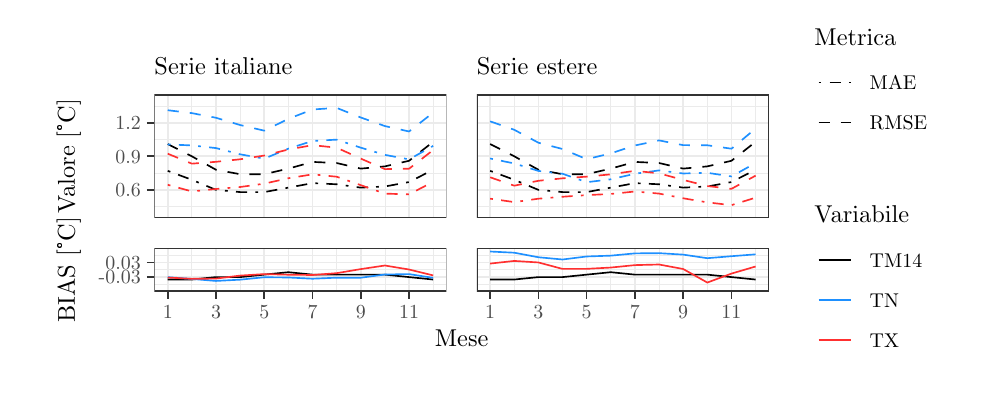
\begin{tikzpicture}[x=1pt,y=1pt]
\definecolor{fillColor}{RGB}{255,255,255}
\path[use as bounding box,fill=fillColor] (0,0) rectangle (341.43,128.04);
\begin{scope}
\path[clip] (  0.00,  0.00) rectangle (341.43,128.04);
\definecolor{drawColor}{RGB}{255,255,255}

\path[draw=drawColor,line width= 0.6pt,line join=round,line cap=round,fill=fillColor] (  0.00,  0.00) rectangle (341.43,128.04);
\end{scope}
\begin{scope}
\path[clip] (  5.50, 53.84) rectangle (156.82,122.54);
\definecolor{drawColor}{RGB}{255,255,255}
\definecolor{fillColor}{RGB}{255,255,255}

\path[draw=drawColor,line width= 0.6pt,line join=round,line cap=round,fill=fillColor] (  5.50, 53.84) rectangle (156.82,122.54);
\end{scope}
\begin{scope}
\path[clip] (156.82, 53.84) rectangle (335.93,122.54);
\definecolor{drawColor}{RGB}{255,255,255}
\definecolor{fillColor}{RGB}{255,255,255}

\path[draw=drawColor,line width= 0.6pt,line join=round,line cap=round,fill=fillColor] (156.82, 53.84) rectangle (335.93,122.54);
\end{scope}
\begin{scope}
\path[clip] (  5.50,  5.50) rectangle (156.82, 53.84);
\definecolor{drawColor}{RGB}{255,255,255}
\definecolor{fillColor}{RGB}{255,255,255}

\path[draw=drawColor,line width= 0.6pt,line join=round,line cap=round,fill=fillColor] (  5.50,  5.50) rectangle (156.82, 53.84);
\end{scope}
\begin{scope}
\path[clip] (156.82,  5.50) rectangle (335.93, 53.84);
\definecolor{drawColor}{RGB}{255,255,255}
\definecolor{fillColor}{RGB}{255,255,255}

\path[draw=drawColor,line width= 0.6pt,line join=round,line cap=round,fill=fillColor] (156.82,  5.50) rectangle (335.93, 53.84);
\end{scope}
\begin{scope}
\path[clip] ( 45.82, 59.34) rectangle (151.32,103.76);
\definecolor{fillColor}{RGB}{255,255,255}

\path[fill=fillColor] ( 45.82, 59.34) rectangle (151.32,103.76);
\definecolor{drawColor}{gray}{0.92}

\path[draw=drawColor,line width= 0.3pt,line join=round] ( 45.82, 63.38) --
	(151.32, 63.38);

\path[draw=drawColor,line width= 0.3pt,line join=round] ( 45.82, 75.49) --
	(151.32, 75.49);

\path[draw=drawColor,line width= 0.3pt,line join=round] ( 45.82, 87.61) --
	(151.32, 87.61);

\path[draw=drawColor,line width= 0.3pt,line join=round] ( 45.82, 99.73) --
	(151.32, 99.73);

\path[draw=drawColor,line width= 0.3pt,line join=round] ( 59.33, 59.34) --
	( 59.33,103.76);

\path[draw=drawColor,line width= 0.3pt,line join=round] ( 76.77, 59.34) --
	( 76.77,103.76);

\path[draw=drawColor,line width= 0.3pt,line join=round] ( 94.21, 59.34) --
	( 94.21,103.76);

\path[draw=drawColor,line width= 0.3pt,line join=round] (111.65, 59.34) --
	(111.65,103.76);

\path[draw=drawColor,line width= 0.3pt,line join=round] (129.09, 59.34) --
	(129.09,103.76);

\path[draw=drawColor,line width= 0.3pt,line join=round] (146.52, 59.34) --
	(146.52,103.76);

\path[draw=drawColor,line width= 0.6pt,line join=round] ( 45.82, 69.43) --
	(151.32, 69.43);

\path[draw=drawColor,line width= 0.6pt,line join=round] ( 45.82, 81.55) --
	(151.32, 81.55);

\path[draw=drawColor,line width= 0.6pt,line join=round] ( 45.82, 93.67) --
	(151.32, 93.67);

\path[draw=drawColor,line width= 0.6pt,line join=round] ( 50.61, 59.34) --
	( 50.61,103.76);

\path[draw=drawColor,line width= 0.6pt,line join=round] ( 68.05, 59.34) --
	( 68.05,103.76);

\path[draw=drawColor,line width= 0.6pt,line join=round] ( 85.49, 59.34) --
	( 85.49,103.76);

\path[draw=drawColor,line width= 0.6pt,line join=round] (102.93, 59.34) --
	(102.93,103.76);

\path[draw=drawColor,line width= 0.6pt,line join=round] (120.37, 59.34) --
	(120.37,103.76);

\path[draw=drawColor,line width= 0.6pt,line join=round] (137.81, 59.34) --
	(137.81,103.76);
\definecolor{drawColor}{RGB}{0,0,0}

\path[draw=drawColor,line width= 0.6pt,dash pattern=on 1pt off 3pt on 4pt off 3pt ,line join=round] ( 50.61, 76.30) --
	( 59.33, 73.07) --
	( 68.05, 69.43) --
	( 76.77, 68.63) --
	( 85.49, 68.63) --
	( 94.21, 70.24) --
	(102.93, 71.86) --
	(111.65, 71.45) --
	(120.37, 70.24) --
	(129.09, 70.65) --
	(137.81, 72.26) --
	(146.52, 76.70);

\path[draw=drawColor,line width= 0.6pt,dash pattern=on 4pt off 4pt ,line join=round] ( 50.61, 85.99) --
	( 59.33, 81.55) --
	( 68.05, 76.70) --
	( 76.77, 75.09) --
	( 85.49, 75.09) --
	( 94.21, 77.11) --
	(102.93, 79.53) --
	(111.65, 79.13) --
	(120.37, 77.11) --
	(129.09, 77.92) --
	(137.81, 79.94) --
	(146.52, 86.80);
\definecolor{drawColor}{RGB}{30,144,255}

\path[draw=drawColor,line width= 0.6pt,dash pattern=on 1pt off 3pt on 4pt off 3pt ,line join=round] ( 50.61, 85.86) --
	( 59.33, 85.49) --
	( 68.05, 84.53) --
	( 76.77, 82.28) --
	( 85.49, 80.71) --
	( 94.21, 84.33) --
	(102.93, 87.10) --
	(111.65, 87.58) --
	(120.37, 84.68) --
	(129.09, 82.08) --
	(137.81, 80.44) --
	(146.52, 85.31);

\path[draw=drawColor,line width= 0.6pt,dash pattern=on 4pt off 4pt ,line join=round] ( 50.61, 98.21) --
	( 59.33, 97.16) --
	( 68.05, 95.48) --
	( 76.77, 92.86) --
	( 85.49, 90.82) --
	( 94.21, 95.09) --
	(102.93, 98.48) --
	(111.65, 99.05) --
	(120.37, 95.58) --
	(129.09, 92.48) --
	(137.81, 90.53) --
	(146.52, 97.33);
\definecolor{drawColor}{RGB}{255,48,48}

\path[draw=drawColor,line width= 0.6pt,dash pattern=on 1pt off 3pt on 4pt off 3pt ,line join=round] ( 50.61, 71.27) --
	( 59.33, 68.86) --
	( 68.05, 69.75) --
	( 76.77, 70.46) --
	( 85.49, 71.67) --
	( 94.21, 73.63) --
	(102.93, 75.04) --
	(111.65, 74.18) --
	(120.37, 71.13) --
	(129.09, 68.07) --
	(137.81, 67.81) --
	(146.52, 72.34);

\path[draw=drawColor,line width= 0.6pt,dash pattern=on 4pt off 4pt ,line join=round] ( 50.61, 82.50) --
	( 59.33, 78.90) --
	( 68.05, 79.57) --
	( 76.77, 80.48) --
	( 85.49, 81.83) --
	( 94.21, 84.02) --
	(102.93, 85.58) --
	(111.65, 84.68) --
	(120.37, 80.72) --
	(129.09, 76.93) --
	(137.81, 77.07) --
	(146.52, 83.82);
\definecolor{drawColor}{gray}{0.20}

\path[draw=drawColor,line width= 0.6pt,line join=round,line cap=round] ( 45.82, 59.34) rectangle (151.32,103.76);
\end{scope}
\begin{scope}
\path[clip] (  0.00,  0.00) rectangle (341.43,128.04);
\definecolor{drawColor}{gray}{0.30}

\node[text=drawColor,anchor=base east,inner sep=0pt, outer sep=0pt, scale=  0.72] at ( 40.87, 66.97) {0.6};

\node[text=drawColor,anchor=base east,inner sep=0pt, outer sep=0pt, scale=  0.72] at ( 40.87, 79.09) {0.9};

\node[text=drawColor,anchor=base east,inner sep=0pt, outer sep=0pt, scale=  0.72] at ( 40.87, 91.20) {1.2};
\end{scope}
\begin{scope}
\path[clip] (  0.00,  0.00) rectangle (341.43,128.04);
\definecolor{drawColor}{gray}{0.20}

\path[draw=drawColor,line width= 0.6pt,line join=round] ( 43.07, 69.43) --
	( 45.82, 69.43);

\path[draw=drawColor,line width= 0.6pt,line join=round] ( 43.07, 81.55) --
	( 45.82, 81.55);

\path[draw=drawColor,line width= 0.6pt,line join=round] ( 43.07, 93.67) --
	( 45.82, 93.67);
\end{scope}
\begin{scope}
\path[clip] (  0.00,  0.00) rectangle (341.43,128.04);
\definecolor{drawColor}{RGB}{0,0,0}

\node[text=drawColor,rotate= 90.00,anchor=base,inner sep=0pt, outer sep=0pt, scale=  0.88] at ( 17.06, 81.55) {Valore [\textdegree C]};
\end{scope}
\begin{scope}
\path[clip] (  0.00,  0.00) rectangle (341.43,128.04);
\definecolor{drawColor}{RGB}{0,0,0}

\node[text=drawColor,anchor=base west,inner sep=0pt, outer sep=0pt, scale=  0.88] at ( 45.82,110.98) {Serie italiane};
\end{scope}
\begin{scope}
\path[clip] (162.32, 59.34) rectangle (267.82,103.76);
\definecolor{fillColor}{RGB}{255,255,255}

\path[fill=fillColor] (162.32, 59.34) rectangle (267.82,103.76);
\definecolor{drawColor}{gray}{0.92}

\path[draw=drawColor,line width= 0.3pt,line join=round] (162.32, 63.38) --
	(267.82, 63.38);

\path[draw=drawColor,line width= 0.3pt,line join=round] (162.32, 75.49) --
	(267.82, 75.49);

\path[draw=drawColor,line width= 0.3pt,line join=round] (162.32, 87.61) --
	(267.82, 87.61);

\path[draw=drawColor,line width= 0.3pt,line join=round] (162.32, 99.73) --
	(267.82, 99.73);

\path[draw=drawColor,line width= 0.3pt,line join=round] (175.84, 59.34) --
	(175.84,103.76);

\path[draw=drawColor,line width= 0.3pt,line join=round] (193.27, 59.34) --
	(193.27,103.76);

\path[draw=drawColor,line width= 0.3pt,line join=round] (210.71, 59.34) --
	(210.71,103.76);

\path[draw=drawColor,line width= 0.3pt,line join=round] (228.15, 59.34) --
	(228.15,103.76);

\path[draw=drawColor,line width= 0.3pt,line join=round] (245.59, 59.34) --
	(245.59,103.76);

\path[draw=drawColor,line width= 0.3pt,line join=round] (263.03, 59.34) --
	(263.03,103.76);

\path[draw=drawColor,line width= 0.6pt,line join=round] (162.32, 69.43) --
	(267.82, 69.43);

\path[draw=drawColor,line width= 0.6pt,line join=round] (162.32, 81.55) --
	(267.82, 81.55);

\path[draw=drawColor,line width= 0.6pt,line join=round] (162.32, 93.67) --
	(267.82, 93.67);

\path[draw=drawColor,line width= 0.6pt,line join=round] (167.12, 59.34) --
	(167.12,103.76);

\path[draw=drawColor,line width= 0.6pt,line join=round] (184.55, 59.34) --
	(184.55,103.76);

\path[draw=drawColor,line width= 0.6pt,line join=round] (201.99, 59.34) --
	(201.99,103.76);

\path[draw=drawColor,line width= 0.6pt,line join=round] (219.43, 59.34) --
	(219.43,103.76);

\path[draw=drawColor,line width= 0.6pt,line join=round] (236.87, 59.34) --
	(236.87,103.76);

\path[draw=drawColor,line width= 0.6pt,line join=round] (254.31, 59.34) --
	(254.31,103.76);
\definecolor{drawColor}{RGB}{0,0,0}

\path[draw=drawColor,line width= 0.6pt,dash pattern=on 1pt off 3pt on 4pt off 3pt ,line join=round] (167.12, 76.30) --
	(175.84, 73.07) --
	(184.55, 69.43) --
	(193.27, 68.63) --
	(201.99, 68.63) --
	(210.71, 70.24) --
	(219.43, 71.86) --
	(228.15, 71.45) --
	(236.87, 70.24) --
	(245.59, 70.65) --
	(254.31, 72.26) --
	(263.03, 76.70);

\path[draw=drawColor,line width= 0.6pt,dash pattern=on 4pt off 4pt ,line join=round] (167.12, 85.99) --
	(175.84, 81.55) --
	(184.55, 76.70) --
	(193.27, 75.09) --
	(201.99, 75.09) --
	(210.71, 77.11) --
	(219.43, 79.53) --
	(228.15, 79.13) --
	(236.87, 77.11) --
	(245.59, 77.92) --
	(254.31, 79.94) --
	(263.03, 86.80);
\definecolor{drawColor}{RGB}{30,144,255}

\path[draw=drawColor,line width= 0.6pt,dash pattern=on 1pt off 3pt on 4pt off 3pt ,line join=round] (167.12, 80.76) --
	(175.84, 78.97) --
	(184.55, 76.28) --
	(193.27, 75.25) --
	(201.99, 72.20) --
	(210.71, 73.25) --
	(219.43, 75.25) --
	(228.15, 76.47) --
	(236.87, 75.35) --
	(245.59, 75.60) --
	(254.31, 74.28) --
	(263.03, 79.13);

\path[draw=drawColor,line width= 0.6pt,dash pattern=on 4pt off 4pt ,line join=round] (167.12, 94.19) --
	(175.84, 91.13) --
	(184.55, 86.47) --
	(193.27, 84.19) --
	(201.99, 80.50) --
	(210.71, 82.63) --
	(219.43, 85.47) --
	(228.15, 87.30) --
	(236.87, 85.59) --
	(245.59, 85.55) --
	(254.31, 84.30) --
	(263.03, 91.58);
\definecolor{drawColor}{RGB}{255,48,48}

\path[draw=drawColor,line width= 0.6pt,dash pattern=on 1pt off 3pt on 4pt off 3pt ,line join=round] (167.12, 66.25) --
	(175.84, 65.00) --
	(184.55, 66.24) --
	(193.27, 66.94) --
	(201.99, 67.54) --
	(210.71, 67.95) --
	(219.43, 68.84) --
	(228.15, 68.09) --
	(236.87, 66.39) --
	(245.59, 64.91) --
	(254.31, 63.91) --
	(263.03, 66.61);

\path[draw=drawColor,line width= 0.6pt,dash pattern=on 4pt off 4pt ,line join=round] (167.12, 73.97) --
	(175.84, 70.94) --
	(184.55, 72.71) --
	(193.27, 73.60) --
	(201.99, 74.21) --
	(210.71, 75.04) --
	(219.43, 76.32) --
	(228.15, 75.40) --
	(236.87, 73.03) --
	(245.59, 70.81) --
	(254.31, 69.80) --
	(263.03, 74.57);
\definecolor{drawColor}{gray}{0.20}

\path[draw=drawColor,line width= 0.6pt,line join=round,line cap=round] (162.32, 59.34) rectangle (267.82,103.76);
\end{scope}
\begin{scope}
\path[clip] (  0.00,  0.00) rectangle (341.43,128.04);
\definecolor{drawColor}{RGB}{0,0,0}

\node[text=drawColor,anchor=base west,inner sep=0pt, outer sep=0pt, scale=  0.88] at (162.32,110.98) {Serie estere};
\end{scope}
\begin{scope}
\path[clip] ( 45.82, 32.79) rectangle (151.32, 48.34);
\definecolor{fillColor}{RGB}{255,255,255}

\path[fill=fillColor] ( 45.82, 32.79) rectangle (151.32, 48.34);
\definecolor{drawColor}{gray}{0.92}

\path[draw=drawColor,line width= 0.3pt,line join=round] ( 45.82, 35.26) --
	(151.32, 35.26);

\path[draw=drawColor,line width= 0.3pt,line join=round] ( 45.82, 40.56) --
	(151.32, 40.56);

\path[draw=drawColor,line width= 0.3pt,line join=round] ( 45.82, 45.86) --
	(151.32, 45.86);

\path[draw=drawColor,line width= 0.3pt,line join=round] ( 59.33, 32.79) --
	( 59.33, 48.34);

\path[draw=drawColor,line width= 0.3pt,line join=round] ( 76.77, 32.79) --
	( 76.77, 48.34);

\path[draw=drawColor,line width= 0.3pt,line join=round] ( 94.21, 32.79) --
	( 94.21, 48.34);

\path[draw=drawColor,line width= 0.3pt,line join=round] (111.65, 32.79) --
	(111.65, 48.34);

\path[draw=drawColor,line width= 0.3pt,line join=round] (129.09, 32.79) --
	(129.09, 48.34);

\path[draw=drawColor,line width= 0.3pt,line join=round] (146.52, 32.79) --
	(146.52, 48.34);

\path[draw=drawColor,line width= 0.6pt,line join=round] ( 45.82, 37.91) --
	(151.32, 37.91);

\path[draw=drawColor,line width= 0.6pt,line join=round] ( 45.82, 43.21) --
	(151.32, 43.21);

\path[draw=drawColor,line width= 0.6pt,line join=round] ( 50.61, 32.79) --
	( 50.61, 48.34);

\path[draw=drawColor,line width= 0.6pt,line join=round] ( 68.05, 32.79) --
	( 68.05, 48.34);

\path[draw=drawColor,line width= 0.6pt,line join=round] ( 85.49, 32.79) --
	( 85.49, 48.34);

\path[draw=drawColor,line width= 0.6pt,line join=round] (102.93, 32.79) --
	(102.93, 48.34);

\path[draw=drawColor,line width= 0.6pt,line join=round] (120.37, 32.79) --
	(120.37, 48.34);

\path[draw=drawColor,line width= 0.6pt,line join=round] (137.81, 32.79) --
	(137.81, 48.34);
\definecolor{drawColor}{RGB}{0,0,0}

\path[draw=drawColor,line width= 0.6pt,line join=round] ( 50.61, 37.03) --
	( 59.33, 37.03) --
	( 68.05, 37.91) --
	( 76.77, 37.91) --
	( 85.49, 38.80) --
	( 94.21, 39.68) --
	(102.93, 38.80) --
	(111.65, 38.80) --
	(120.37, 38.80) --
	(129.09, 38.80) --
	(137.81, 37.91) --
	(146.52, 37.03);
\definecolor{drawColor}{RGB}{30,144,255}

\path[draw=drawColor,line width= 0.6pt,line join=round] ( 50.61, 37.89) --
	( 59.33, 37.24) --
	( 68.05, 36.52) --
	( 76.77, 36.98) --
	( 85.49, 37.86) --
	( 94.21, 37.77) --
	(102.93, 37.32) --
	(111.65, 37.70) --
	(120.37, 37.69) --
	(129.09, 38.85) --
	(137.81, 38.99) --
	(146.52, 37.64);
\definecolor{drawColor}{RGB}{255,48,48}

\path[draw=drawColor,line width= 0.6pt,line join=round] ( 50.61, 37.75) --
	( 59.33, 37.28) --
	( 68.05, 37.37) --
	( 76.77, 38.45) --
	( 85.49, 39.00) --
	( 94.21, 38.77) --
	(102.93, 38.67) --
	(111.65, 39.33) --
	(120.37, 40.80) --
	(129.09, 42.10) --
	(137.81, 40.65) --
	(146.52, 38.52);
\definecolor{drawColor}{gray}{0.20}

\path[draw=drawColor,line width= 0.6pt,line join=round,line cap=round] ( 45.82, 32.79) rectangle (151.32, 48.34);
\end{scope}
\begin{scope}
\path[clip] (  0.00,  0.00) rectangle (341.43,128.04);
\definecolor{drawColor}{gray}{0.30}

\node[text=drawColor,anchor=base east,inner sep=0pt, outer sep=0pt, scale=  0.72] at ( 40.87, 35.45) {-0.03};

\node[text=drawColor,anchor=base east,inner sep=0pt, outer sep=0pt, scale=  0.72] at ( 40.87, 40.75) {0.03};
\end{scope}
\begin{scope}
\path[clip] (  0.00,  0.00) rectangle (341.43,128.04);
\definecolor{drawColor}{gray}{0.20}

\path[draw=drawColor,line width= 0.6pt,line join=round] ( 43.07, 37.91) --
	( 45.82, 37.91);

\path[draw=drawColor,line width= 0.6pt,line join=round] ( 43.07, 43.21) --
	( 45.82, 43.21);
\end{scope}
\begin{scope}
\path[clip] (  0.00,  0.00) rectangle (341.43,128.04);
\definecolor{drawColor}{gray}{0.20}

\path[draw=drawColor,line width= 0.6pt,line join=round] ( 50.61, 30.04) --
	( 50.61, 32.79);

\path[draw=drawColor,line width= 0.6pt,line join=round] ( 68.05, 30.04) --
	( 68.05, 32.79);

\path[draw=drawColor,line width= 0.6pt,line join=round] ( 85.49, 30.04) --
	( 85.49, 32.79);

\path[draw=drawColor,line width= 0.6pt,line join=round] (102.93, 30.04) --
	(102.93, 32.79);

\path[draw=drawColor,line width= 0.6pt,line join=round] (120.37, 30.04) --
	(120.37, 32.79);

\path[draw=drawColor,line width= 0.6pt,line join=round] (137.81, 30.04) --
	(137.81, 32.79);
\end{scope}
\begin{scope}
\path[clip] (  0.00,  0.00) rectangle (341.43,128.04);
\definecolor{drawColor}{gray}{0.30}

\node[text=drawColor,anchor=base,inner sep=0pt, outer sep=0pt, scale=  0.72] at ( 50.61, 22.91) {1};

\node[text=drawColor,anchor=base,inner sep=0pt, outer sep=0pt, scale=  0.72] at ( 68.05, 22.91) {3};

\node[text=drawColor,anchor=base,inner sep=0pt, outer sep=0pt, scale=  0.72] at ( 85.49, 22.91) {5};

\node[text=drawColor,anchor=base,inner sep=0pt, outer sep=0pt, scale=  0.72] at (102.93, 22.91) {7};

\node[text=drawColor,anchor=base,inner sep=0pt, outer sep=0pt, scale=  0.72] at (120.37, 22.91) {9};

\node[text=drawColor,anchor=base,inner sep=0pt, outer sep=0pt, scale=  0.72] at (137.81, 22.91) {11};
\end{scope}
\begin{scope}
\path[clip] (  0.00,  0.00) rectangle (341.43,128.04);
\definecolor{drawColor}{RGB}{0,0,0}

\node[text=drawColor,rotate= 90.00,anchor=base,inner sep=0pt, outer sep=0pt, scale=  0.88] at ( 17.06, 40.56) {BIAS [\textdegree C]};
\end{scope}
\begin{scope}
\path[clip] (162.32, 32.79) rectangle (267.82, 48.34);
\definecolor{fillColor}{RGB}{255,255,255}

\path[fill=fillColor] (162.32, 32.79) rectangle (267.82, 48.34);
\definecolor{drawColor}{gray}{0.92}

\path[draw=drawColor,line width= 0.3pt,line join=round] (162.32, 35.26) --
	(267.82, 35.26);

\path[draw=drawColor,line width= 0.3pt,line join=round] (162.32, 40.56) --
	(267.82, 40.56);

\path[draw=drawColor,line width= 0.3pt,line join=round] (162.32, 45.86) --
	(267.82, 45.86);

\path[draw=drawColor,line width= 0.3pt,line join=round] (175.84, 32.79) --
	(175.84, 48.34);

\path[draw=drawColor,line width= 0.3pt,line join=round] (193.27, 32.79) --
	(193.27, 48.34);

\path[draw=drawColor,line width= 0.3pt,line join=round] (210.71, 32.79) --
	(210.71, 48.34);

\path[draw=drawColor,line width= 0.3pt,line join=round] (228.15, 32.79) --
	(228.15, 48.34);

\path[draw=drawColor,line width= 0.3pt,line join=round] (245.59, 32.79) --
	(245.59, 48.34);

\path[draw=drawColor,line width= 0.3pt,line join=round] (263.03, 32.79) --
	(263.03, 48.34);

\path[draw=drawColor,line width= 0.6pt,line join=round] (162.32, 37.91) --
	(267.82, 37.91);

\path[draw=drawColor,line width= 0.6pt,line join=round] (162.32, 43.21) --
	(267.82, 43.21);

\path[draw=drawColor,line width= 0.6pt,line join=round] (167.12, 32.79) --
	(167.12, 48.34);

\path[draw=drawColor,line width= 0.6pt,line join=round] (184.55, 32.79) --
	(184.55, 48.34);

\path[draw=drawColor,line width= 0.6pt,line join=round] (201.99, 32.79) --
	(201.99, 48.34);

\path[draw=drawColor,line width= 0.6pt,line join=round] (219.43, 32.79) --
	(219.43, 48.34);

\path[draw=drawColor,line width= 0.6pt,line join=round] (236.87, 32.79) --
	(236.87, 48.34);

\path[draw=drawColor,line width= 0.6pt,line join=round] (254.31, 32.79) --
	(254.31, 48.34);
\definecolor{drawColor}{RGB}{0,0,0}

\path[draw=drawColor,line width= 0.6pt,line join=round] (167.12, 37.03) --
	(175.84, 37.03) --
	(184.55, 37.91) --
	(193.27, 37.91) --
	(201.99, 38.80) --
	(210.71, 39.68) --
	(219.43, 38.80) --
	(228.15, 38.80) --
	(236.87, 38.80) --
	(245.59, 38.80) --
	(254.31, 37.91) --
	(263.03, 37.03);
\definecolor{drawColor}{RGB}{30,144,255}

\path[draw=drawColor,line width= 0.6pt,line join=round] (167.12, 47.15) --
	(175.84, 46.72) --
	(184.55, 45.08) --
	(193.27, 44.27) --
	(201.99, 45.36) --
	(210.71, 45.66) --
	(219.43, 46.48) --
	(228.15, 46.56) --
	(236.87, 46.03) --
	(245.59, 44.74) --
	(254.31, 45.46) --
	(263.03, 46.13);
\definecolor{drawColor}{RGB}{255,48,48}

\path[draw=drawColor,line width= 0.6pt,line join=round] (167.12, 42.80) --
	(175.84, 43.75) --
	(184.55, 43.20) --
	(193.27, 40.87) --
	(201.99, 40.89) --
	(210.71, 41.36) --
	(219.43, 42.24) --
	(228.15, 42.46) --
	(236.87, 40.83) --
	(245.59, 35.94) --
	(254.31, 39.18) --
	(263.03, 41.74);
\definecolor{drawColor}{gray}{0.20}

\path[draw=drawColor,line width= 0.6pt,line join=round,line cap=round] (162.32, 32.79) rectangle (267.82, 48.34);
\end{scope}
\begin{scope}
\path[clip] (  0.00,  0.00) rectangle (341.43,128.04);
\definecolor{drawColor}{gray}{0.20}

\path[draw=drawColor,line width= 0.6pt,line join=round] (167.12, 30.04) --
	(167.12, 32.79);

\path[draw=drawColor,line width= 0.6pt,line join=round] (184.55, 30.04) --
	(184.55, 32.79);

\path[draw=drawColor,line width= 0.6pt,line join=round] (201.99, 30.04) --
	(201.99, 32.79);

\path[draw=drawColor,line width= 0.6pt,line join=round] (219.43, 30.04) --
	(219.43, 32.79);

\path[draw=drawColor,line width= 0.6pt,line join=round] (236.87, 30.04) --
	(236.87, 32.79);

\path[draw=drawColor,line width= 0.6pt,line join=round] (254.31, 30.04) --
	(254.31, 32.79);
\end{scope}
\begin{scope}
\path[clip] (  0.00,  0.00) rectangle (341.43,128.04);
\definecolor{drawColor}{gray}{0.30}

\node[text=drawColor,anchor=base,inner sep=0pt, outer sep=0pt, scale=  0.72] at (167.12, 22.91) {1};

\node[text=drawColor,anchor=base,inner sep=0pt, outer sep=0pt, scale=  0.72] at (184.55, 22.91) {3};

\node[text=drawColor,anchor=base,inner sep=0pt, outer sep=0pt, scale=  0.72] at (201.99, 22.91) {5};

\node[text=drawColor,anchor=base,inner sep=0pt, outer sep=0pt, scale=  0.72] at (219.43, 22.91) {7};

\node[text=drawColor,anchor=base,inner sep=0pt, outer sep=0pt, scale=  0.72] at (236.87, 22.91) {9};

\node[text=drawColor,anchor=base,inner sep=0pt, outer sep=0pt, scale=  0.72] at (254.31, 22.91) {11};
\end{scope}
\begin{scope}
\path[clip] (  0.00,  0.00) rectangle (341.43,128.04);
\definecolor{drawColor}{RGB}{0,0,0}

\node[text=drawColor,anchor=base,inner sep=0pt, outer sep=0pt, scale=  0.88] at (156.82, 12.71) {Mese};
\end{scope}
\begin{scope}
\path[clip] (  0.00,  0.00) rectangle (341.43,128.04);
\definecolor{fillColor}{RGB}{255,255,255}

\path[fill=fillColor] (278.82, 81.00) rectangle (330.43,134.18);
\end{scope}
\begin{scope}
\path[clip] (  0.00,  0.00) rectangle (341.43,128.04);
\definecolor{drawColor}{RGB}{0,0,0}

\node[text=drawColor,anchor=base west,inner sep=0pt, outer sep=0pt, scale=  0.88] at (284.32,121.77) {Metrica};
\end{scope}
\begin{scope}
\path[clip] (  0.00,  0.00) rectangle (341.43,128.04);
\definecolor{fillColor}{RGB}{255,255,255}

\path[fill=fillColor] (284.32,100.96) rectangle (298.78,115.41);
\end{scope}
\begin{scope}
\path[clip] (  0.00,  0.00) rectangle (341.43,128.04);
\definecolor{drawColor}{RGB}{0,0,0}

\path[draw=drawColor,line width= 0.6pt,dash pattern=on 1pt off 3pt on 4pt off 3pt ,line join=round] (285.77,108.18) -- (297.33,108.18);
\end{scope}
\begin{scope}
\path[clip] (  0.00,  0.00) rectangle (341.43,128.04);
\definecolor{fillColor}{RGB}{255,255,255}

\path[fill=fillColor] (284.32, 86.50) rectangle (298.78,100.96);
\end{scope}
\begin{scope}
\path[clip] (  0.00,  0.00) rectangle (341.43,128.04);
\definecolor{drawColor}{RGB}{0,0,0}

\path[draw=drawColor,line width= 0.6pt,dash pattern=on 4pt off 4pt ,line join=round] (285.77, 93.73) -- (297.33, 93.73);
\end{scope}
\begin{scope}
\path[clip] (  0.00,  0.00) rectangle (341.43,128.04);
\definecolor{drawColor}{RGB}{0,0,0}

\node[text=drawColor,anchor=base west,inner sep=0pt, outer sep=0pt, scale=  0.72] at (304.28,105.72) {MAE};
\end{scope}
\begin{scope}
\path[clip] (  0.00,  0.00) rectangle (341.43,128.04);
\definecolor{drawColor}{RGB}{0,0,0}

\node[text=drawColor,anchor=base west,inner sep=0pt, outer sep=0pt, scale=  0.72] at (304.28, 91.27) {RMSE};
\end{scope}
\begin{scope}
\path[clip] (  0.00,  0.00) rectangle (341.43,128.04);
\definecolor{fillColor}{RGB}{255,255,255}

\path[fill=fillColor] (278.82,  2.37) rectangle (328.65, 70.00);
\end{scope}
\begin{scope}
\path[clip] (  0.00,  0.00) rectangle (341.43,128.04);
\definecolor{drawColor}{RGB}{0,0,0}

\node[text=drawColor,anchor=base west,inner sep=0pt, outer sep=0pt, scale=  0.88] at (284.32, 57.59) {Variabile};
\end{scope}
\begin{scope}
\path[clip] (  0.00,  0.00) rectangle (341.43,128.04);
\definecolor{fillColor}{RGB}{255,255,255}

\path[fill=fillColor] (284.32, 36.78) rectangle (298.78, 51.23);
\end{scope}
\begin{scope}
\path[clip] (  0.00,  0.00) rectangle (341.43,128.04);
\definecolor{drawColor}{RGB}{0,0,0}

\path[draw=drawColor,line width= 0.6pt,line join=round] (285.77, 44.00) -- (297.33, 44.00);
\end{scope}
\begin{scope}
\path[clip] (  0.00,  0.00) rectangle (341.43,128.04);
\definecolor{fillColor}{RGB}{255,255,255}

\path[fill=fillColor] (284.32, 22.32) rectangle (298.78, 36.78);
\end{scope}
\begin{scope}
\path[clip] (  0.00,  0.00) rectangle (341.43,128.04);
\definecolor{drawColor}{RGB}{30,144,255}

\path[draw=drawColor,line width= 0.6pt,line join=round] (285.77, 29.55) -- (297.33, 29.55);
\end{scope}
\begin{scope}
\path[clip] (  0.00,  0.00) rectangle (341.43,128.04);
\definecolor{fillColor}{RGB}{255,255,255}

\path[fill=fillColor] (284.32,  7.87) rectangle (298.78, 22.32);
\end{scope}
\begin{scope}
\path[clip] (  0.00,  0.00) rectangle (341.43,128.04);
\definecolor{drawColor}{RGB}{255,48,48}

\path[draw=drawColor,line width= 0.6pt,line join=round] (285.77, 15.10) -- (297.33, 15.10);
\end{scope}
\begin{scope}
\path[clip] (  0.00,  0.00) rectangle (341.43,128.04);
\definecolor{drawColor}{RGB}{0,0,0}

\node[text=drawColor,anchor=base west,inner sep=0pt, outer sep=0pt, scale=  0.72] at (304.28, 41.54) {TM14};
\end{scope}
\begin{scope}
\path[clip] (  0.00,  0.00) rectangle (341.43,128.04);
\definecolor{drawColor}{RGB}{0,0,0}

\node[text=drawColor,anchor=base west,inner sep=0pt, outer sep=0pt, scale=  0.72] at (304.28, 27.09) {TN};
\end{scope}
\begin{scope}
\path[clip] (  0.00,  0.00) rectangle (341.43,128.04);
\definecolor{drawColor}{RGB}{0,0,0}

\node[text=drawColor,anchor=base west,inner sep=0pt, outer sep=0pt, scale=  0.72] at (304.28, 12.63) {TX};
\end{scope}
\end{tikzpicture}

  \caption{Confronto tra le statistiche del 2014 e le serie italiane ed estere del dataset prodotto.}\label{fig:diffs-mese-ita}
\end{figure}
La tabella~\ref{tab:diffs-mese-ita} e la figura~\ref{fig:diffs-mese-ita} mostrano le statistiche degli scostamenti del modello per le stazioni del centro-nord Italia, che indicano un consistente scarto tra la capacità del modello di ricostruire le serie di temperature minime rispetto alle massime, in particolare nei mesi estivi ed invernali. Ciononostante il bias rimane sempre entro il margine accettabile di \(\pm\qty{0.05}{\degreeCelsius}\). Gli scostamenti assoluti e quadratici delle minime invece sono considerevolmente più alti, a suggerire che rispetto al precedente dataset c'è una maggiore presenza di outliers che non vengono ricostruiti in maniera efficace.

\begin{table}[ht]
  \centering
  \begin{adjustbox}{max width=\textwidth}
    \begin{threeparttable}
      \caption{Accuratezza delle climatologie stimate per le temperature minime e massime delle stazioni francesi, svizzere, austriache e slovene.}\label{tab:bias-non-ita}
      
\begin{tabular}[t]{rrrrrrrrrr}
\toprule
\multicolumn{1}{c}{ } & \multicolumn{3}{c}{TN} & \multicolumn{3}{c}{TX} & \multicolumn{3}{c}{2014\tnote{*}} \\
\cmidrule(l{3pt}r{3pt}){2-4} \cmidrule(l{3pt}r{3pt}){5-7} \cmidrule(l{3pt}r{3pt}){8-10}
Mese & BIAS & MAE & RMSE & BIAS & MAE & RMSE & BIAS & MAE & RMSE\\
\midrule
1 & 0.07 & 0.88 & 1.21 & 0.03 & 0.52 & 0.71 & -0.04 & 0.77 & 1.01\\
2 & 0.07 & 0.84 & 1.14 & 0.04 & 0.49 & 0.64 & -0.04 & 0.69 & 0.90\\
3 & 0.05 & 0.77 & 1.02 & 0.03 & 0.52 & 0.68 & -0.03 & 0.60 & 0.78\\
4 & 0.04 & 0.74 & 0.97 & 0.00 & 0.54 & 0.70 & -0.03 & 0.58 & 0.74\\
5 & 0.05 & 0.67 & 0.87 & 0.00 & 0.55 & 0.72 & -0.02 & 0.58 & 0.74\\
\addlinespace
6 & 0.06 & 0.69 & 0.93 & 0.01 & 0.56 & 0.74 & -0.01 & 0.62 & 0.79\\
7 & 0.07 & 0.74 & 1.00 & 0.02 & 0.59 & 0.77 & -0.02 & 0.66 & 0.85\\
8 & 0.07 & 0.77 & 1.04 & 0.02 & 0.57 & 0.75 & -0.02 & 0.65 & 0.84\\
9 & 0.06 & 0.75 & 1.00 & 0.00 & 0.52 & 0.69 & -0.02 & 0.62 & 0.79\\
10 & 0.05 & 0.75 & 1.00 & -0.05 & 0.49 & 0.63 & -0.02 & 0.63 & 0.81\\
\addlinespace
11 & 0.06 & 0.72 & 0.97 & -0.02 & 0.46 & 0.61 & -0.03 & 0.67 & 0.86\\
12 & 0.06 & 0.84 & 1.15 & 0.01 & 0.53 & 0.73 & -0.04 & 0.78 & 1.03\\
\bottomrule
\end{tabular}
      \begin{tablenotes}
      \item[*] Tabella 1 da~\cite[p.~10]{brunettiHighresolutionTemperatureClimatology2014}. Le statistiche d'errore riguardano le temperature medie per il trentennio 1961--1990 e l'intera penisola.
      \end{tablenotes}
    \end{threeparttable}
  \end{adjustbox}
\end{table}
La situazione è differente se si considerano le stazioni esterne al territorio italiano: in questo caso i bias delle minime sono marcatamente più importanti, probabilmente a causa della maggiore proporzione di stazioni in alta quota di queste regioni. Gli scostamenti assoluti e quadratici sono invece inferiori, indicando che ci sono meno ricostruzioni molto anomale.

È stata poi contrallata la presenza di errori sistematici nella procedura di ricostruzione a livello locale. In particolare, vista la numerosa quantità di sorgenti presenti nel dataset, è stata fatta una statistica sulle serie raggruppandole per regione di appartenenza. Il pannello sinistro della figura~\ref{fig:boxplots-ita} mostra come alcuni territori (in particolare Liguria, Lombardia, Piemonte, Toscana e Valle d'Aosta) contribuiscano in maniera più significativa a bias e varianza complessivi. Essendo territori dall'orografia complessa, si è studiata la dipendenza del bias dalla quota: il pannello destro della stessa figura mostra che per le minime lo scostamento complessivo è correlato alla quota, mentre per le massime ne aumenta la dispersione, fino a divenire più importante rispetto a quella delle minime.

\begin{figure}[ht]
  \centering
  % Created by tikzDevice version 0.12.6 on 2025-04-07 20:16:07
% !TEX encoding = UTF-8 Unicode
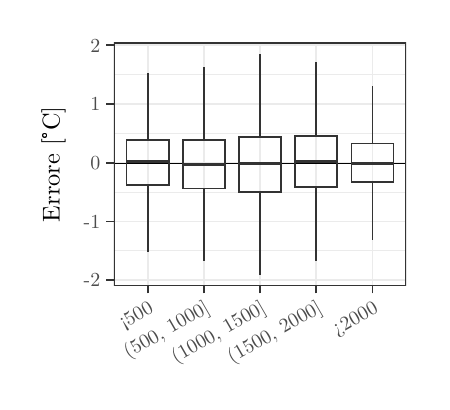
\begin{tikzpicture}[x=1pt,y=1pt]
\definecolor{fillColor}{RGB}{255,255,255}
\path[use as bounding box,fill=fillColor] (0,0) rectangle (142.26,128.04);
\begin{scope}
\path[clip] (  0.00,  0.00) rectangle (142.26,128.04);
\definecolor{drawColor}{RGB}{255,255,255}

\path[draw=drawColor,line width= 0.6pt,line join=round,line cap=round,fill=fillColor] (  0.00,  0.00) rectangle (142.26,128.04);
\end{scope}
\begin{scope}
\path[clip] ( 31.18, 34.79) rectangle (136.76,122.54);
\definecolor{fillColor}{RGB}{255,255,255}

\path[fill=fillColor] ( 31.18, 34.79) rectangle (136.76,122.54);
\definecolor{drawColor}{gray}{0.92}

\path[draw=drawColor,line width= 0.3pt,line join=round] ( 31.18, 47.41) --
	(136.76, 47.41);

\path[draw=drawColor,line width= 0.3pt,line join=round] ( 31.18, 68.63) --
	(136.76, 68.63);

\path[draw=drawColor,line width= 0.3pt,line join=round] ( 31.18, 89.84) --
	(136.76, 89.84);

\path[draw=drawColor,line width= 0.3pt,line join=round] ( 31.18,111.06) --
	(136.76,111.06);

\path[draw=drawColor,line width= 0.6pt,line join=round] ( 31.18, 36.80) --
	(136.76, 36.80);

\path[draw=drawColor,line width= 0.6pt,line join=round] ( 31.18, 58.02) --
	(136.76, 58.02);

\path[draw=drawColor,line width= 0.6pt,line join=round] ( 31.18, 79.24) --
	(136.76, 79.24);

\path[draw=drawColor,line width= 0.6pt,line join=round] ( 31.18,100.45) --
	(136.76,100.45);

\path[draw=drawColor,line width= 0.6pt,line join=round] ( 31.18,121.67) --
	(136.76,121.67);

\path[draw=drawColor,line width= 0.6pt,line join=round] ( 43.36, 34.79) --
	( 43.36,122.54);

\path[draw=drawColor,line width= 0.6pt,line join=round] ( 63.67, 34.79) --
	( 63.67,122.54);

\path[draw=drawColor,line width= 0.6pt,line join=round] ( 83.97, 34.79) --
	( 83.97,122.54);

\path[draw=drawColor,line width= 0.6pt,line join=round] (104.28, 34.79) --
	(104.28,122.54);

\path[draw=drawColor,line width= 0.6pt,line join=round] (124.58, 34.79) --
	(124.58,122.54);
\definecolor{drawColor}{RGB}{0,0,0}

\path[draw=drawColor,line width= 0.1pt,line join=round] ( 31.18, 79.24) -- (136.76, 79.24);
\definecolor{drawColor}{gray}{0.20}

\path[draw=drawColor,line width= 0.6pt,line join=round] ( 43.36, 87.36) -- ( 43.36,111.63);

\path[draw=drawColor,line width= 0.6pt,line join=round] ( 43.36, 71.17) -- ( 43.36, 46.90);

\path[draw=drawColor,line width= 0.6pt] ( 35.75, 87.36) --
	( 35.75, 71.17) --
	( 50.98, 71.17) --
	( 50.98, 87.36) --
	( 35.75, 87.36) --
	cycle;

\path[draw=drawColor,line width= 1.1pt] ( 35.75, 79.57) -- ( 50.98, 79.57);

\path[draw=drawColor,line width= 0.6pt,line join=round] ( 63.67, 87.47) -- ( 63.67,113.78);

\path[draw=drawColor,line width= 0.6pt,line join=round] ( 63.67, 69.89) -- ( 63.67, 43.61);

\path[draw=drawColor,line width= 0.6pt] ( 56.05, 87.47) --
	( 56.05, 69.89) --
	( 71.28, 69.89) --
	( 71.28, 87.47) --
	( 56.05, 87.47) --
	cycle;

\path[draw=drawColor,line width= 1.1pt] ( 56.05, 78.47) -- ( 71.28, 78.47);

\path[draw=drawColor,line width= 0.6pt,line join=round] ( 83.97, 88.64) -- ( 83.97,118.55);

\path[draw=drawColor,line width= 0.6pt,line join=round] ( 83.97, 68.69) -- ( 83.97, 38.78);

\path[draw=drawColor,line width= 0.6pt] ( 76.36, 88.64) --
	( 76.36, 68.69) --
	( 91.59, 68.69) --
	( 91.59, 88.64) --
	( 76.36, 88.64) --
	cycle;

\path[draw=drawColor,line width= 1.1pt] ( 76.36, 78.95) -- ( 91.59, 78.95);

\path[draw=drawColor,line width= 0.6pt,line join=round] (104.28, 88.85) -- (104.28,115.71);

\path[draw=drawColor,line width= 0.6pt,line join=round] (104.28, 70.56) -- (104.28, 43.57);

\path[draw=drawColor,line width= 0.6pt] ( 96.66, 88.85) --
	( 96.66, 70.56) --
	(111.89, 70.56) --
	(111.89, 88.85) --
	( 96.66, 88.85) --
	cycle;

\path[draw=drawColor,line width= 1.1pt] ( 96.66, 79.54) -- (111.89, 79.54);

\path[draw=drawColor,line width= 0.6pt,line join=round] (124.58, 86.24) -- (124.58,106.88);

\path[draw=drawColor,line width= 0.6pt,line join=round] (124.58, 72.27) -- (124.58, 51.46);

\path[draw=drawColor,line width= 0.6pt] (116.97, 86.24) --
	(116.97, 72.27) --
	(132.20, 72.27) --
	(132.20, 86.24) --
	(116.97, 86.24) --
	cycle;

\path[draw=drawColor,line width= 1.1pt] (116.97, 79.11) -- (132.20, 79.11);

\path[draw=drawColor,line width= 0.6pt,line join=round,line cap=round] ( 31.18, 34.79) rectangle (136.76,122.54);
\end{scope}
\begin{scope}
\path[clip] (  0.00,  0.00) rectangle (142.26,128.04);
\definecolor{drawColor}{gray}{0.30}

\node[text=drawColor,anchor=base east,inner sep=0pt, outer sep=0pt, scale=  0.72] at ( 26.23, 34.34) {-2};

\node[text=drawColor,anchor=base east,inner sep=0pt, outer sep=0pt, scale=  0.72] at ( 26.23, 55.56) {-1};

\node[text=drawColor,anchor=base east,inner sep=0pt, outer sep=0pt, scale=  0.72] at ( 26.23, 76.77) {0};

\node[text=drawColor,anchor=base east,inner sep=0pt, outer sep=0pt, scale=  0.72] at ( 26.23, 97.99) {1};

\node[text=drawColor,anchor=base east,inner sep=0pt, outer sep=0pt, scale=  0.72] at ( 26.23,119.20) {2};
\end{scope}
\begin{scope}
\path[clip] (  0.00,  0.00) rectangle (142.26,128.04);
\definecolor{drawColor}{gray}{0.20}

\path[draw=drawColor,line width= 0.6pt,line join=round] ( 28.43, 36.80) --
	( 31.18, 36.80);

\path[draw=drawColor,line width= 0.6pt,line join=round] ( 28.43, 58.02) --
	( 31.18, 58.02);

\path[draw=drawColor,line width= 0.6pt,line join=round] ( 28.43, 79.24) --
	( 31.18, 79.24);

\path[draw=drawColor,line width= 0.6pt,line join=round] ( 28.43,100.45) --
	( 31.18,100.45);

\path[draw=drawColor,line width= 0.6pt,line join=round] ( 28.43,121.67) --
	( 31.18,121.67);
\end{scope}
\begin{scope}
\path[clip] (  0.00,  0.00) rectangle (142.26,128.04);
\definecolor{drawColor}{gray}{0.20}

\path[draw=drawColor,line width= 0.6pt,line join=round] ( 43.36, 32.04) --
	( 43.36, 34.79);

\path[draw=drawColor,line width= 0.6pt,line join=round] ( 63.67, 32.04) --
	( 63.67, 34.79);

\path[draw=drawColor,line width= 0.6pt,line join=round] ( 83.97, 32.04) --
	( 83.97, 34.79);

\path[draw=drawColor,line width= 0.6pt,line join=round] (104.28, 32.04) --
	(104.28, 34.79);

\path[draw=drawColor,line width= 0.6pt,line join=round] (124.58, 32.04) --
	(124.58, 34.79);
\end{scope}
\begin{scope}
\path[clip] (  0.00,  0.00) rectangle (142.26,128.04);
\definecolor{drawColor}{gray}{0.30}

\node[text=drawColor,rotate= 30.00,anchor=base east,inner sep=0pt, outer sep=0pt, scale=  0.72] at ( 45.83, 25.57) {<500};

\node[text=drawColor,rotate= 30.00,anchor=base east,inner sep=0pt, outer sep=0pt, scale=  0.72] at ( 66.13, 25.57) {(500, 1000]};

\node[text=drawColor,rotate= 30.00,anchor=base east,inner sep=0pt, outer sep=0pt, scale=  0.72] at ( 86.44, 25.57) {(1000, 1500]};

\node[text=drawColor,rotate= 30.00,anchor=base east,inner sep=0pt, outer sep=0pt, scale=  0.72] at (106.74, 25.57) {(1500, 2000]};

\node[text=drawColor,rotate= 30.00,anchor=base east,inner sep=0pt, outer sep=0pt, scale=  0.72] at (127.04, 25.57) {>2000};
\end{scope}
\begin{scope}
\path[clip] (  0.00,  0.00) rectangle (142.26,128.04);
\definecolor{drawColor}{RGB}{0,0,0}

\node[text=drawColor,rotate= 90.00,anchor=base,inner sep=0pt, outer sep=0pt, scale=  0.88] at ( 11.56, 78.66) {Errore [\textdegree C]};
\end{scope}
\end{tikzpicture}

  \caption{Distribuzioni dei bias del modello a seconda della regione e di diverse fasce di quota.}\label{fig:boxplots-ita}
\end{figure}

Infine, è stato analizzato il legame tra BIAS e distanza dal mare delle serie a bassa quota (inferiore a \qty{500}{\meter}). La figura~\ref{fig:sea-bias} mostra come le stazioni costiere siano ricostruite con una certa difficoltà rispetto alle altre, in particolare con BIAS e RMSE significativi per le temperature minime e marcato effetto stagionale per le massime. Rispetto al lavoro del 2014 si è scelto di considerare ``vicine'' stazioni a meno di \qty{10}{\kilo\meter}, piuttosto che \qty{1.3}{\kilo\meter}, in modo da avere un campione di circa 400 stazioni.

\begin{figure}[ht]
  \centering
  % Created by tikzDevice version 0.12.6 on 2025-04-07 03:17:30
% !TEX encoding = UTF-8 Unicode
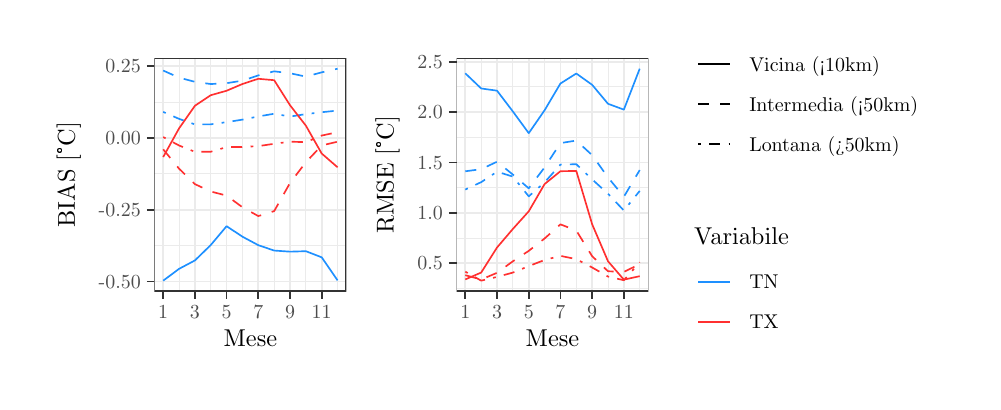
\begin{tikzpicture}[x=1pt,y=1pt]
\definecolor{fillColor}{RGB}{255,255,255}
\path[use as bounding box,fill=fillColor] (0,0) rectangle (341.43,128.04);
\begin{scope}
\path[clip] (  0.00,  0.00) rectangle (341.43,128.04);
\definecolor{drawColor}{RGB}{255,255,255}

\path[draw=drawColor,line width= 0.6pt,line join=round,line cap=round,fill=fillColor] (  0.00,  0.00) rectangle (341.43,128.04);
\end{scope}
\begin{scope}
\path[clip] (  5.50,  5.50) rectangle (120.63,122.54);
\definecolor{drawColor}{RGB}{255,255,255}
\definecolor{fillColor}{RGB}{255,255,255}

\path[draw=drawColor,line width= 0.6pt,line join=round,line cap=round,fill=fillColor] (  5.50,  5.50) rectangle (120.63,122.54);
\end{scope}
\begin{scope}
\path[clip] (120.63,  5.50) rectangle (335.93,122.54);
\definecolor{drawColor}{RGB}{255,255,255}
\definecolor{fillColor}{RGB}{255,255,255}

\path[draw=drawColor,line width= 0.6pt,line join=round,line cap=round,fill=fillColor] (120.63,  5.50) rectangle (335.93,122.54);
\end{scope}
\begin{scope}
\path[clip] ( 45.82, 32.79) rectangle (115.13,117.04);
\definecolor{fillColor}{RGB}{255,255,255}

\path[fill=fillColor] ( 45.82, 32.79) rectangle (115.13,117.04);
\definecolor{drawColor}{gray}{0.92}

\path[draw=drawColor,line width= 0.3pt,line join=round] ( 45.82, 49.27) --
	(115.13, 49.27);

\path[draw=drawColor,line width= 0.3pt,line join=round] ( 45.82, 75.22) --
	(115.13, 75.22);

\path[draw=drawColor,line width= 0.3pt,line join=round] ( 45.82,101.17) --
	(115.13,101.17);

\path[draw=drawColor,line width= 0.3pt,line join=round] ( 54.70, 32.79) --
	( 54.70,117.04);

\path[draw=drawColor,line width= 0.3pt,line join=round] ( 66.15, 32.79) --
	( 66.15,117.04);

\path[draw=drawColor,line width= 0.3pt,line join=round] ( 77.61, 32.79) --
	( 77.61,117.04);

\path[draw=drawColor,line width= 0.3pt,line join=round] ( 89.07, 32.79) --
	( 89.07,117.04);

\path[draw=drawColor,line width= 0.3pt,line join=round] (100.53, 32.79) --
	(100.53,117.04);

\path[draw=drawColor,line width= 0.3pt,line join=round] (111.98, 32.79) --
	(111.98,117.04);

\path[draw=drawColor,line width= 0.6pt,line join=round] ( 45.82, 36.30) --
	(115.13, 36.30);

\path[draw=drawColor,line width= 0.6pt,line join=round] ( 45.82, 62.25) --
	(115.13, 62.25);

\path[draw=drawColor,line width= 0.6pt,line join=round] ( 45.82, 88.20) --
	(115.13, 88.20);

\path[draw=drawColor,line width= 0.6pt,line join=round] ( 45.82,114.15) --
	(115.13,114.15);

\path[draw=drawColor,line width= 0.6pt,line join=round] ( 48.97, 32.79) --
	( 48.97,117.04);

\path[draw=drawColor,line width= 0.6pt,line join=round] ( 60.43, 32.79) --
	( 60.43,117.04);

\path[draw=drawColor,line width= 0.6pt,line join=round] ( 71.88, 32.79) --
	( 71.88,117.04);

\path[draw=drawColor,line width= 0.6pt,line join=round] ( 83.34, 32.79) --
	( 83.34,117.04);

\path[draw=drawColor,line width= 0.6pt,line join=round] ( 94.80, 32.79) --
	( 94.80,117.04);

\path[draw=drawColor,line width= 0.6pt,line join=round] (106.25, 32.79) --
	(106.25,117.04);
\definecolor{drawColor}{RGB}{30,144,255}

\path[draw=drawColor,line width= 0.6pt,line join=round] ( 48.97, 36.62) --
	( 54.70, 40.89) --
	( 60.43, 43.93) --
	( 66.15, 49.49) --
	( 71.88, 56.31) --
	( 77.61, 52.51) --
	( 83.34, 49.45) --
	( 89.07, 47.50) --
	( 94.80, 47.10) --
	(100.53, 47.27) --
	(106.25, 45.05) --
	(111.98, 36.73);

\path[draw=drawColor,line width= 0.6pt,dash pattern=on 4pt off 4pt ,line join=round] ( 48.97,112.54) --
	( 54.70,109.99) --
	( 60.43,108.47) --
	( 66.15,107.67) --
	( 71.88,107.98) --
	( 77.61,108.90) --
	( 83.34,110.80) --
	( 89.07,112.26) --
	( 94.80,111.58) --
	(100.53,110.35) --
	(106.25,111.90) --
	(111.98,113.21);

\path[draw=drawColor,line width= 0.6pt,dash pattern=on 1pt off 3pt on 4pt off 3pt ,line join=round] ( 48.97, 97.60) --
	( 54.70, 95.09) --
	( 60.43, 93.09) --
	( 66.15, 93.11) --
	( 71.88, 93.90) --
	( 77.61, 94.81) --
	( 83.34, 95.96) --
	( 89.07, 96.94) --
	( 94.80, 95.92) --
	(100.53, 96.80) --
	(106.25, 97.49) --
	(111.98, 98.08);
\definecolor{drawColor}{RGB}{255,48,48}

\path[draw=drawColor,line width= 0.6pt,line join=round] ( 48.97, 81.30) --
	( 54.70, 91.64) --
	( 60.43, 99.81) --
	( 66.15,103.63) --
	( 71.88,105.25) --
	( 77.61,107.69) --
	( 83.34,109.57) --
	( 89.07,109.06) --
	( 94.80,100.01) --
	(100.53, 92.63) --
	(106.25, 82.56) --
	(111.98, 77.59);

\path[draw=drawColor,line width= 0.6pt,dash pattern=on 4pt off 4pt ,line join=round] ( 48.97, 84.08) --
	( 54.70, 77.09) --
	( 60.43, 71.51) --
	( 66.15, 68.84) --
	( 71.88, 67.36) --
	( 77.61, 63.14) --
	( 83.34, 59.96) --
	( 89.07, 61.75) --
	( 94.80, 71.93) --
	(100.53, 79.42) --
	(106.25, 85.48) --
	(111.98, 86.84);

\path[draw=drawColor,line width= 0.6pt,dash pattern=on 1pt off 3pt on 4pt off 3pt ,line join=round] ( 48.97, 88.51) --
	( 54.70, 85.47) --
	( 60.43, 83.18) --
	( 66.15, 83.21) --
	( 71.88, 84.88) --
	( 77.61, 84.95) --
	( 83.34, 85.24) --
	( 89.07, 86.08) --
	( 94.80, 86.85) --
	(100.53, 86.66) --
	(106.25, 89.06) --
	(111.98, 90.27);
\definecolor{drawColor}{gray}{0.20}

\path[draw=drawColor,line width= 0.6pt,line join=round,line cap=round] ( 45.82, 32.79) rectangle (115.13,117.04);
\end{scope}
\begin{scope}
\path[clip] (  0.00,  0.00) rectangle (341.43,128.04);
\definecolor{drawColor}{gray}{0.30}

\node[text=drawColor,anchor=base east,inner sep=0pt, outer sep=0pt, scale=  0.72] at ( 40.87, 33.84) {-0.50};

\node[text=drawColor,anchor=base east,inner sep=0pt, outer sep=0pt, scale=  0.72] at ( 40.87, 59.79) {-0.25};

\node[text=drawColor,anchor=base east,inner sep=0pt, outer sep=0pt, scale=  0.72] at ( 40.87, 85.74) {0.00};

\node[text=drawColor,anchor=base east,inner sep=0pt, outer sep=0pt, scale=  0.72] at ( 40.87,111.68) {0.25};
\end{scope}
\begin{scope}
\path[clip] (  0.00,  0.00) rectangle (341.43,128.04);
\definecolor{drawColor}{gray}{0.20}

\path[draw=drawColor,line width= 0.6pt,line join=round] ( 43.07, 36.30) --
	( 45.82, 36.30);

\path[draw=drawColor,line width= 0.6pt,line join=round] ( 43.07, 62.25) --
	( 45.82, 62.25);

\path[draw=drawColor,line width= 0.6pt,line join=round] ( 43.07, 88.20) --
	( 45.82, 88.20);

\path[draw=drawColor,line width= 0.6pt,line join=round] ( 43.07,114.15) --
	( 45.82,114.15);
\end{scope}
\begin{scope}
\path[clip] (  0.00,  0.00) rectangle (341.43,128.04);
\definecolor{drawColor}{gray}{0.20}

\path[draw=drawColor,line width= 0.6pt,line join=round] ( 48.97, 30.04) --
	( 48.97, 32.79);

\path[draw=drawColor,line width= 0.6pt,line join=round] ( 60.43, 30.04) --
	( 60.43, 32.79);

\path[draw=drawColor,line width= 0.6pt,line join=round] ( 71.88, 30.04) --
	( 71.88, 32.79);

\path[draw=drawColor,line width= 0.6pt,line join=round] ( 83.34, 30.04) --
	( 83.34, 32.79);

\path[draw=drawColor,line width= 0.6pt,line join=round] ( 94.80, 30.04) --
	( 94.80, 32.79);

\path[draw=drawColor,line width= 0.6pt,line join=round] (106.25, 30.04) --
	(106.25, 32.79);
\end{scope}
\begin{scope}
\path[clip] (  0.00,  0.00) rectangle (341.43,128.04);
\definecolor{drawColor}{gray}{0.30}

\node[text=drawColor,anchor=base,inner sep=0pt, outer sep=0pt, scale=  0.72] at ( 48.97, 22.91) {1};

\node[text=drawColor,anchor=base,inner sep=0pt, outer sep=0pt, scale=  0.72] at ( 60.43, 22.91) {3};

\node[text=drawColor,anchor=base,inner sep=0pt, outer sep=0pt, scale=  0.72] at ( 71.88, 22.91) {5};

\node[text=drawColor,anchor=base,inner sep=0pt, outer sep=0pt, scale=  0.72] at ( 83.34, 22.91) {7};

\node[text=drawColor,anchor=base,inner sep=0pt, outer sep=0pt, scale=  0.72] at ( 94.80, 22.91) {9};

\node[text=drawColor,anchor=base,inner sep=0pt, outer sep=0pt, scale=  0.72] at (106.25, 22.91) {11};
\end{scope}
\begin{scope}
\path[clip] (  0.00,  0.00) rectangle (341.43,128.04);
\definecolor{drawColor}{RGB}{0,0,0}

\node[text=drawColor,anchor=base,inner sep=0pt, outer sep=0pt, scale=  0.88] at ( 80.48, 12.71) {Mese};
\end{scope}
\begin{scope}
\path[clip] (  0.00,  0.00) rectangle (341.43,128.04);
\definecolor{drawColor}{RGB}{0,0,0}

\node[text=drawColor,rotate= 90.00,anchor=base,inner sep=0pt, outer sep=0pt, scale=  0.88] at ( 17.06, 74.91) {BIAS [\textdegree C]};
\end{scope}
\begin{scope}
\path[clip] (154.99, 32.79) rectangle (224.31,117.04);
\definecolor{fillColor}{RGB}{255,255,255}

\path[fill=fillColor] (154.99, 32.79) rectangle (224.31,117.04);
\definecolor{drawColor}{gray}{0.92}

\path[draw=drawColor,line width= 0.3pt,line join=round] (154.99, 33.85) --
	(224.31, 33.85);

\path[draw=drawColor,line width= 0.3pt,line join=round] (154.99, 52.05) --
	(224.31, 52.05);

\path[draw=drawColor,line width= 0.3pt,line join=round] (154.99, 70.25) --
	(224.31, 70.25);

\path[draw=drawColor,line width= 0.3pt,line join=round] (154.99, 88.45) --
	(224.31, 88.45);

\path[draw=drawColor,line width= 0.3pt,line join=round] (154.99,106.64) --
	(224.31,106.64);

\path[draw=drawColor,line width= 0.3pt,line join=round] (163.87, 32.79) --
	(163.87,117.04);

\path[draw=drawColor,line width= 0.3pt,line join=round] (175.33, 32.79) --
	(175.33,117.04);

\path[draw=drawColor,line width= 0.3pt,line join=round] (186.79, 32.79) --
	(186.79,117.04);

\path[draw=drawColor,line width= 0.3pt,line join=round] (198.24, 32.79) --
	(198.24,117.04);

\path[draw=drawColor,line width= 0.3pt,line join=round] (209.70, 32.79) --
	(209.70,117.04);

\path[draw=drawColor,line width= 0.3pt,line join=round] (221.16, 32.79) --
	(221.16,117.04);

\path[draw=drawColor,line width= 0.6pt,line join=round] (154.99, 42.95) --
	(224.31, 42.95);

\path[draw=drawColor,line width= 0.6pt,line join=round] (154.99, 61.15) --
	(224.31, 61.15);

\path[draw=drawColor,line width= 0.6pt,line join=round] (154.99, 79.35) --
	(224.31, 79.35);

\path[draw=drawColor,line width= 0.6pt,line join=round] (154.99, 97.54) --
	(224.31, 97.54);

\path[draw=drawColor,line width= 0.6pt,line join=round] (154.99,115.74) --
	(224.31,115.74);

\path[draw=drawColor,line width= 0.6pt,line join=round] (158.14, 32.79) --
	(158.14,117.04);

\path[draw=drawColor,line width= 0.6pt,line join=round] (169.60, 32.79) --
	(169.60,117.04);

\path[draw=drawColor,line width= 0.6pt,line join=round] (181.06, 32.79) --
	(181.06,117.04);

\path[draw=drawColor,line width= 0.6pt,line join=round] (192.51, 32.79) --
	(192.51,117.04);

\path[draw=drawColor,line width= 0.6pt,line join=round] (203.97, 32.79) --
	(203.97,117.04);

\path[draw=drawColor,line width= 0.6pt,line join=round] (215.43, 32.79) --
	(215.43,117.04);
\definecolor{drawColor}{RGB}{30,144,255}

\path[draw=drawColor,line width= 0.6pt,line join=round] (158.14,111.54) --
	(163.87,106.07) --
	(169.60,105.27) --
	(175.33, 97.75) --
	(181.06, 89.92) --
	(186.79, 98.20) --
	(192.51,107.86) --
	(198.24,111.48) --
	(203.97,107.39) --
	(209.70,100.54) --
	(215.43, 98.42) --
	(221.16,113.21);

\path[draw=drawColor,line width= 0.6pt,dash pattern=on 4pt off 4pt ,line join=round] (158.14, 76.14) --
	(163.87, 76.91) --
	(169.60, 79.60) --
	(175.33, 74.95) --
	(181.06, 69.98) --
	(186.79, 77.56) --
	(192.51, 86.33) --
	(198.24, 87.25) --
	(203.97, 81.97) --
	(209.70, 73.93) --
	(215.43, 66.94) --
	(221.16, 76.58);

\path[draw=drawColor,line width= 0.6pt,dash pattern=on 1pt off 3pt on 4pt off 3pt ,line join=round] (158.14, 69.54) --
	(163.87, 72.22) --
	(169.60, 76.00) --
	(175.33, 74.22) --
	(181.06, 67.09) --
	(186.79, 72.14) --
	(192.51, 78.56) --
	(198.24, 78.70) --
	(203.97, 73.22) --
	(209.70, 68.03) --
	(215.43, 61.97) --
	(221.16, 69.05);
\definecolor{drawColor}{RGB}{255,48,48}

\path[draw=drawColor,line width= 0.6pt,line join=round] (158.14, 37.07) --
	(163.87, 39.55) --
	(169.60, 48.60) --
	(175.33, 55.32) --
	(181.06, 61.67) --
	(186.79, 71.53) --
	(192.51, 76.17) --
	(198.24, 76.27) --
	(203.97, 57.01) --
	(209.70, 43.63) --
	(215.43, 36.99) --
	(221.16, 38.24);

\path[draw=drawColor,line width= 0.6pt,dash pattern=on 4pt off 4pt ,line join=round] (158.14, 38.60) --
	(163.87, 37.03) --
	(169.60, 39.46) --
	(175.33, 43.63) --
	(181.06, 47.39) --
	(186.79, 51.86) --
	(192.51, 56.97) --
	(198.24, 54.74) --
	(203.97, 45.46) --
	(209.70, 40.02) --
	(215.43, 39.77) --
	(221.16, 42.60);

\path[draw=drawColor,line width= 0.6pt,dash pattern=on 1pt off 3pt on 4pt off 3pt ,line join=round] (158.14, 39.87) --
	(163.87, 36.62) --
	(169.60, 37.98) --
	(175.33, 39.54) --
	(181.06, 41.88) --
	(186.79, 44.10) --
	(192.51, 45.58) --
	(198.24, 44.41) --
	(203.97, 41.38) --
	(209.70, 38.10) --
	(215.43, 36.78) --
	(221.16, 43.26);
\definecolor{drawColor}{gray}{0.20}

\path[draw=drawColor,line width= 0.6pt,line join=round,line cap=round] (154.99, 32.79) rectangle (224.31,117.04);
\end{scope}
\begin{scope}
\path[clip] (  0.00,  0.00) rectangle (341.43,128.04);
\definecolor{drawColor}{gray}{0.30}

\node[text=drawColor,anchor=base east,inner sep=0pt, outer sep=0pt, scale=  0.72] at (150.04, 40.49) {0.5};

\node[text=drawColor,anchor=base east,inner sep=0pt, outer sep=0pt, scale=  0.72] at (150.04, 58.68) {1.0};

\node[text=drawColor,anchor=base east,inner sep=0pt, outer sep=0pt, scale=  0.72] at (150.04, 76.88) {1.5};

\node[text=drawColor,anchor=base east,inner sep=0pt, outer sep=0pt, scale=  0.72] at (150.04, 95.08) {2.0};

\node[text=drawColor,anchor=base east,inner sep=0pt, outer sep=0pt, scale=  0.72] at (150.04,113.28) {2.5};
\end{scope}
\begin{scope}
\path[clip] (  0.00,  0.00) rectangle (341.43,128.04);
\definecolor{drawColor}{gray}{0.20}

\path[draw=drawColor,line width= 0.6pt,line join=round] (152.24, 42.95) --
	(154.99, 42.95);

\path[draw=drawColor,line width= 0.6pt,line join=round] (152.24, 61.15) --
	(154.99, 61.15);

\path[draw=drawColor,line width= 0.6pt,line join=round] (152.24, 79.35) --
	(154.99, 79.35);

\path[draw=drawColor,line width= 0.6pt,line join=round] (152.24, 97.54) --
	(154.99, 97.54);

\path[draw=drawColor,line width= 0.6pt,line join=round] (152.24,115.74) --
	(154.99,115.74);
\end{scope}
\begin{scope}
\path[clip] (  0.00,  0.00) rectangle (341.43,128.04);
\definecolor{drawColor}{gray}{0.20}

\path[draw=drawColor,line width= 0.6pt,line join=round] (158.14, 30.04) --
	(158.14, 32.79);

\path[draw=drawColor,line width= 0.6pt,line join=round] (169.60, 30.04) --
	(169.60, 32.79);

\path[draw=drawColor,line width= 0.6pt,line join=round] (181.06, 30.04) --
	(181.06, 32.79);

\path[draw=drawColor,line width= 0.6pt,line join=round] (192.51, 30.04) --
	(192.51, 32.79);

\path[draw=drawColor,line width= 0.6pt,line join=round] (203.97, 30.04) --
	(203.97, 32.79);

\path[draw=drawColor,line width= 0.6pt,line join=round] (215.43, 30.04) --
	(215.43, 32.79);
\end{scope}
\begin{scope}
\path[clip] (  0.00,  0.00) rectangle (341.43,128.04);
\definecolor{drawColor}{gray}{0.30}

\node[text=drawColor,anchor=base,inner sep=0pt, outer sep=0pt, scale=  0.72] at (158.14, 22.91) {1};

\node[text=drawColor,anchor=base,inner sep=0pt, outer sep=0pt, scale=  0.72] at (169.60, 22.91) {3};

\node[text=drawColor,anchor=base,inner sep=0pt, outer sep=0pt, scale=  0.72] at (181.06, 22.91) {5};

\node[text=drawColor,anchor=base,inner sep=0pt, outer sep=0pt, scale=  0.72] at (192.51, 22.91) {7};

\node[text=drawColor,anchor=base,inner sep=0pt, outer sep=0pt, scale=  0.72] at (203.97, 22.91) {9};

\node[text=drawColor,anchor=base,inner sep=0pt, outer sep=0pt, scale=  0.72] at (215.43, 22.91) {11};
\end{scope}
\begin{scope}
\path[clip] (  0.00,  0.00) rectangle (341.43,128.04);
\definecolor{drawColor}{RGB}{0,0,0}

\node[text=drawColor,anchor=base,inner sep=0pt, outer sep=0pt, scale=  0.88] at (189.65, 12.71) {Mese};
\end{scope}
\begin{scope}
\path[clip] (  0.00,  0.00) rectangle (341.43,128.04);
\definecolor{drawColor}{RGB}{0,0,0}

\node[text=drawColor,rotate= 90.00,anchor=base,inner sep=0pt, outer sep=0pt, scale=  0.88] at (132.20, 74.91) {RMSE [\textdegree C]};
\end{scope}
\begin{scope}
\path[clip] (  0.00,  0.00) rectangle (341.43,128.04);
\definecolor{fillColor}{RGB}{255,255,255}

\path[fill=fillColor] (235.31, 73.19) rectangle (330.43,140.82);
\end{scope}
\begin{scope}
\path[clip] (  0.00,  0.00) rectangle (341.43,128.04);
\definecolor{drawColor}{RGB}{0,0,0}

\node[text=drawColor,anchor=base west,inner sep=0pt, outer sep=0pt, scale=  0.88] at (240.81,128.40) {Distanza dal mare};
\end{scope}
\begin{scope}
\path[clip] (  0.00,  0.00) rectangle (341.43,128.04);
\definecolor{fillColor}{RGB}{255,255,255}

\path[fill=fillColor] (240.81,107.59) rectangle (255.26,122.05);
\end{scope}
\begin{scope}
\path[clip] (  0.00,  0.00) rectangle (341.43,128.04);
\definecolor{drawColor}{RGB}{0,0,0}

\path[draw=drawColor,line width= 0.6pt,line join=round] (242.25,114.82) -- (253.82,114.82);
\end{scope}
\begin{scope}
\path[clip] (  0.00,  0.00) rectangle (341.43,128.04);
\definecolor{fillColor}{RGB}{255,255,255}

\path[fill=fillColor] (240.81, 93.14) rectangle (255.26,107.59);
\end{scope}
\begin{scope}
\path[clip] (  0.00,  0.00) rectangle (341.43,128.04);
\definecolor{drawColor}{RGB}{0,0,0}

\path[draw=drawColor,line width= 0.6pt,dash pattern=on 4pt off 4pt ,line join=round] (242.25,100.37) -- (253.82,100.37);
\end{scope}
\begin{scope}
\path[clip] (  0.00,  0.00) rectangle (341.43,128.04);
\definecolor{fillColor}{RGB}{255,255,255}

\path[fill=fillColor] (240.81, 78.69) rectangle (255.26, 93.14);
\end{scope}
\begin{scope}
\path[clip] (  0.00,  0.00) rectangle (341.43,128.04);
\definecolor{drawColor}{RGB}{0,0,0}

\path[draw=drawColor,line width= 0.6pt,dash pattern=on 1pt off 3pt on 4pt off 3pt ,line join=round] (242.25, 85.91) -- (253.82, 85.91);
\end{scope}
\begin{scope}
\path[clip] (  0.00,  0.00) rectangle (341.43,128.04);
\definecolor{drawColor}{RGB}{0,0,0}

\node[text=drawColor,anchor=base west,inner sep=0pt, outer sep=0pt, scale=  0.72] at (260.76,112.36) {Vicina (<10km)};
\end{scope}
\begin{scope}
\path[clip] (  0.00,  0.00) rectangle (341.43,128.04);
\definecolor{drawColor}{RGB}{0,0,0}

\node[text=drawColor,anchor=base west,inner sep=0pt, outer sep=0pt, scale=  0.72] at (260.76, 97.90) {Intermedia (<50km)};
\end{scope}
\begin{scope}
\path[clip] (  0.00,  0.00) rectangle (341.43,128.04);
\definecolor{drawColor}{RGB}{0,0,0}

\node[text=drawColor,anchor=base west,inner sep=0pt, outer sep=0pt, scale=  0.72] at (260.76, 83.45) {Lontana (>50km)};
\end{scope}
\begin{scope}
\path[clip] (  0.00,  0.00) rectangle (341.43,128.04);
\definecolor{fillColor}{RGB}{255,255,255}

\path[fill=fillColor] (235.31,  9.00) rectangle (280.55, 62.19);
\end{scope}
\begin{scope}
\path[clip] (  0.00,  0.00) rectangle (341.43,128.04);
\definecolor{drawColor}{RGB}{0,0,0}

\node[text=drawColor,anchor=base west,inner sep=0pt, outer sep=0pt, scale=  0.88] at (240.81, 49.77) {Variabile};
\end{scope}
\begin{scope}
\path[clip] (  0.00,  0.00) rectangle (341.43,128.04);
\definecolor{fillColor}{RGB}{255,255,255}

\path[fill=fillColor] (240.81, 28.96) rectangle (255.26, 43.41);
\end{scope}
\begin{scope}
\path[clip] (  0.00,  0.00) rectangle (341.43,128.04);
\definecolor{drawColor}{RGB}{30,144,255}

\path[draw=drawColor,line width= 0.6pt,line join=round] (242.25, 36.19) -- (253.82, 36.19);
\end{scope}
\begin{scope}
\path[clip] (  0.00,  0.00) rectangle (341.43,128.04);
\definecolor{fillColor}{RGB}{255,255,255}

\path[fill=fillColor] (240.81, 14.50) rectangle (255.26, 28.96);
\end{scope}
\begin{scope}
\path[clip] (  0.00,  0.00) rectangle (341.43,128.04);
\definecolor{drawColor}{RGB}{255,48,48}

\path[draw=drawColor,line width= 0.6pt,line join=round] (242.25, 21.73) -- (253.82, 21.73);
\end{scope}
\begin{scope}
\path[clip] (  0.00,  0.00) rectangle (341.43,128.04);
\definecolor{drawColor}{RGB}{0,0,0}

\node[text=drawColor,anchor=base west,inner sep=0pt, outer sep=0pt, scale=  0.72] at (260.76, 33.72) {TN};
\end{scope}
\begin{scope}
\path[clip] (  0.00,  0.00) rectangle (341.43,128.04);
\definecolor{drawColor}{RGB}{0,0,0}

\node[text=drawColor,anchor=base west,inner sep=0pt, outer sep=0pt, scale=  0.72] at (260.76, 19.27) {TX};
\end{scope}
\end{tikzpicture}

  \caption{BIAS e RMSE delle stazioni italiane in funzione della distanza dal mare (quota < \qty{500}{\meter}).}\label{fig:sea-bias}
\end{figure}
